\documentclass[11pt,a4paper]{article}

\usepackage[T1]{fontenc}
\usepackage[utf8]{inputenc}
\usepackage[margin=1in]{geometry}
\usepackage{graphicx}
\usepackage{listings}
\usepackage{xcolor}
\usepackage{parskip}
\usepackage{float}
\usepackage[hidelinks]{hyperref}
\usepackage{longtable}
\usepackage{array}

% ---------------------------------------------------------------
% Listings setup for LLVM IR
% ---------------------------------------------------------------
\definecolor{irkeyword}{RGB}{0,0,180}
\definecolor{irtype}{RGB}{0,120,0}
\definecolor{ircomment}{RGB}{128,128,128}
\definecolor{irback}{RGB}{246,246,246}

\lstdefinelanguage{LLVM}{
  morekeywords={
    alloca,load,store,getelementptr,icmp,fcmp,add,fdiv,br,switch,phi,call,
    ret,sext,sitofp,select,fpext,define,label,inbounds,volatile,align,nsw,
    nuw,slt,eq,oeq,true,false,void,preds,insertelement,shufflevector,
    extractelement
  },
  morekeywords=[2]{i1,i8,i32,i64,ptr,float,double},
  sensitive=true,
  morecomment=[l]{;},
  morestring=[b]",
}

\lstset{
  language=LLVM,
  basicstyle=\ttfamily\small,
  keywordstyle=\color{irkeyword}\bfseries,
  keywordstyle=[2]\color{irtype},
  commentstyle=\color{ircomment}\itshape,
  backgroundcolor=\color{irback},
  frame=single,
  rulecolor=\color{black!25},
  framesep=5pt,
  xleftmargin=6pt,
  xrightmargin=6pt,
  breaklines=true,
  showstringspaces=false,
  columns=fullflexible,
  keepspaces=true,
}

% Inline IR snippet
\newcommand{\ir}[1]{\texttt{#1}}

\begin{document}

\hypersetup{pageanchor=false}
\begin{titlepage}
\centering
\vspace*{1.2cm}

{
\includegraphics[width=4.2cm]{iitd.png}}

\vspace{1.0cm}

{\huge\scshape Indian Institute of Technology Delhi\par}

\vspace{0.4cm}

\vspace{2.2cm}

{\rule{0.85\textwidth}{0.8pt}\par}
\vspace{0.6cm}
{\LARGE\bfseries COL 729 Lab 2: IR and Compiler Passes\par}
\vspace{0.6cm}
{\rule{0.85\textwidth}{0.8pt}\par}

\vspace{2.5cm}

\begin{minipage}{0.45\textwidth}
\centering
{\Large\bfseries Submitted by}\par
\vspace{0.25cm}
{\large Aditya Anand and Varun Subramaniam\par}
{\large 2023CS50284 and 2023CS50497\par}
\end{minipage}%
\begin{minipage}{0.45\textwidth}
\centering
{\Large\bfseries Instructor}\par
\vspace{0.25cm}
{\Large Prof.\ Sorav Bansal\par}
\end{minipage}

\vfill

{\Large 9 September 2026\par}

\vspace{1cm}

\end{titlepage}
\hypersetup{pageanchor=true}
\pagenumbering{arabic}

\section*{Machines used}

Parts A and B were done on one machine. Parts C and D were
done on another. The two Homebrew LLVM installs are not the
same version.

\textbf{Parts A and B.} Apple M3, arm64 macOS. \texttt{opt} and
\texttt{clang} were Homebrew LLVM 23.1.0.

\begin{lstlisting}[language={}]
Homebrew LLVM version 23.1.0
Optimized build.
Default target: arm64-apple-darwin25.5.0
Host CPU: apple-m3
\end{lstlisting}

\textbf{Parts C and D.} Apple M1, arm64 macOS. \texttt{opt} and
\texttt{clang} were Homebrew LLVM 18.1.8.

\begin{lstlisting}[language={}]
Homebrew LLVM version 18.1.8
Optimized build.
Default target: arm64-apple-darwin25.5.0
Host CPU: apple-m1
\end{lstlisting}

\section{Part A}

All except \texttt{select} are taken from \texttt{opcodes.O0.ll}.
\texttt{select} is from \texttt{opcodes.canonical.ll}.

\subsection*{\texttt{alloca}}

\begin{lstlisting}
13: %1 = alloca i32, align 4
\end{lstlisting}

This line creates a space for a 32-bit integer on the stack (for
\texttt{compiletimeindex}) and \texttt{\%1} is its address. The result type is
\texttt{ptr}.

\subsection*{\texttt{load}}

\begin{lstlisting}
16: %3 = load volatile i32, ptr @runtimeindex, align 4
\end{lstlisting}

This line loads a 32-bit integer \emph{from} \texttt{@runtimeindex} and writes
that value into the SSA name \texttt{\%3}. It does not store into
\texttt{runtimeindex}. The result type is \texttt{i32}.

\subsection*{\texttt{store}}

\begin{lstlisting}
15: store i32 0, ptr %1, align 4
\end{lstlisting}

This stores the value \texttt{0} into the memory that \texttt{\%1} points to
(\texttt{compiletimeindex}). \texttt{\%1} is only the address and it does not
change. \texttt{store} has no result.

\subsection*{\texttt{getelementptr}}

\begin{lstlisting}
18: %5 = getelementptr inbounds [2 x %struct.myStruct], ptr %2, i64 0, i64 %4
\end{lstlisting}

\texttt{\%2} gives the base address of the \texttt{myStruct} array. The first
\texttt{i64 0} moves the pointer by 0 distance forward and changes the pointing
type from a hypothetical array of \texttt{[2 x \%struct.myStruct]} and points to a
\texttt{[2 x \%struct.myStruct]} without moving. The second \texttt{i64 \%4} does pointer
arithmetic with the offset stored in \texttt{\%4} and adds that as offset, so
\texttt{\%5} is the required address. The result type is \texttt{ptr}. This is done in
the line \texttt{arr[runtimeindex].scalar = 1}.
The getelementptr arithmetic is purely done on the addresses. There is no memory access involved. The memory access is done by a separate load/store. Hence, getelementptr does not read the memory.

\subsection*{\texttt{icmp}}

\begin{lstlisting}
46: %5 = icmp slt i32 %4, 3
\end{lstlisting}

This is for integer comparison. It sets \texttt{\%5} to true if \texttt{\%4}
is less than 3. That is the loop continuation test \texttt{i < 3} in
\texttt{f2}: true keeps going around the loop, false leaves it. It is
not the \texttt{break}. The result type is \texttt{i1}.

\subsection*{\texttt{fcmp}}

\begin{lstlisting}
67: %18 = fcmp oeq double %17, 2.000000e+00
\end{lstlisting}

\texttt{oeq} means neither operand is NaN and the two values are equal.
The C is \texttt{else if (myf == 2.0) break;} in \texttt{f2}. The
literal is \texttt{2.0}, a \texttt{double}, so \texttt{myf} is first
widened with \texttt{fpext} and then compared as
\texttt{fcmp oeq double}. That is why this is not a float compare
against \texttt{2.0f}. The result type is \texttt{i1}.

\subsection*{\texttt{add}}

\begin{lstlisting}
51: %8 = add nsw i32 %7, 1
\end{lstlisting}

\texttt{nsw} means no signed wrap, meaning that no overflow will take place. In
this line 1 is added to \texttt{\%7} to get \texttt{\%8}.

This is the \texttt{loopcarried += 1} step inside the loop in \texttt{f2}.
\texttt{\%7} is the value loaded from \texttt{loopcarried} on line 50. The result
type is \texttt{i32}.

\subsection*{\texttt{fdiv}}

\begin{lstlisting}
55: %11 = fdiv float %10, 2.000000e+00
\end{lstlisting}

The float division value of \texttt{\%10} divided by \texttt{2.0f} is stored in
\texttt{\%11} as done in \texttt{f2}. The result type is \texttt{float}.

\subsection*{\texttt{br}}

\begin{lstlisting}
42: br label %3
\end{lstlisting}

This is the jump from the start of \texttt{f2} into the loop header of
\texttt{for (int i = 0; i < 3; i++)}. The header is block \texttt{\%3}.
\texttt{br} has no result.

\subsection*{\texttt{switch}}

\begin{lstlisting}
101: switch i32 %6, label %31 [
\end{lstlisting}

This is \texttt{switch(a)} in \texttt{f3}. \texttt{\%6} is the loaded
value of \texttt{a}. If no case matches, control goes to block
\texttt{\%31}, the join after the switch. \texttt{switch} has no result.

\subsection*{\texttt{phi}}

\begin{lstlisting}
120: %16 = phi i32 [ %13, %12 ], [ 7, %14 ]
\end{lstlisting}

It changes this line \texttt{int t = (runtimeindex > 1) ? loopcarried : 7;}.
Clang emits it as 4 basic blocks \texttt{\%9}, \texttt{\%12}, \texttt{\%14}, \texttt{\%15}; the phi
does not create them. The phi sits at the join block \texttt{\%15} and picks \texttt{\%13}
if control came from \texttt{\%12} and 7 if it came from \texttt{\%14}, so that SSA is not
broken. The result type is \texttt{i32}.

\subsection*{\texttt{call}}

\begin{lstlisting}
104: call void @f1()
\end{lstlisting}

Calls the function \texttt{f1}. It is the first case of the switch. \texttt{f1}
returns void so there is no result.

\subsection*{\texttt{ret}}

\begin{lstlisting}
34: ret void
\end{lstlisting}

This is the implicit return at the end of void \texttt{f1}. There is no
\texttt{return} keyword in the C; clang still emits \texttt{ret void}.
\texttt{ret} has no result.

\subsection*{\texttt{sext}}

\begin{lstlisting}
17: %4 = sext i32 %3 to i64
\end{lstlisting}

It is a \texttt{sext} (signed extension) of the value of \texttt{\%3} from 32 to 64
bits because pointer arithmetic is done in 64 bits. The result type is
\texttt{i64}.

\subsection*{\texttt{sitofp}}

\begin{lstlisting}
54: %10 = sitofp i32 %9 to float
\end{lstlisting}

It is used in this line \texttt{float myf = loopcarried/2.0f;}. \texttt{\%9} is the
\texttt{loopcarried} value, which is converted into a float register \texttt{\%10}
before doing arithmetic. The result type is \texttt{float}.

\subsection*{\texttt{select}}

\begin{lstlisting}
71: %4 = select i1 %2, i32 %3, i32 7
\end{lstlisting}

It changes this line \texttt{int t = (runtimeindex > 1) ? loopcarried : 7;}.
Instead of using 2 basic blocks to first calculate the values and using phi, it
is storing the result of the comparison in \texttt{\%2} and using its result directly
to take from one of the branches. The result type is \texttt{i32}.

\subsection*{Control flow graph of \texttt{f2}}

\begin{figure}[H]
  \centering
  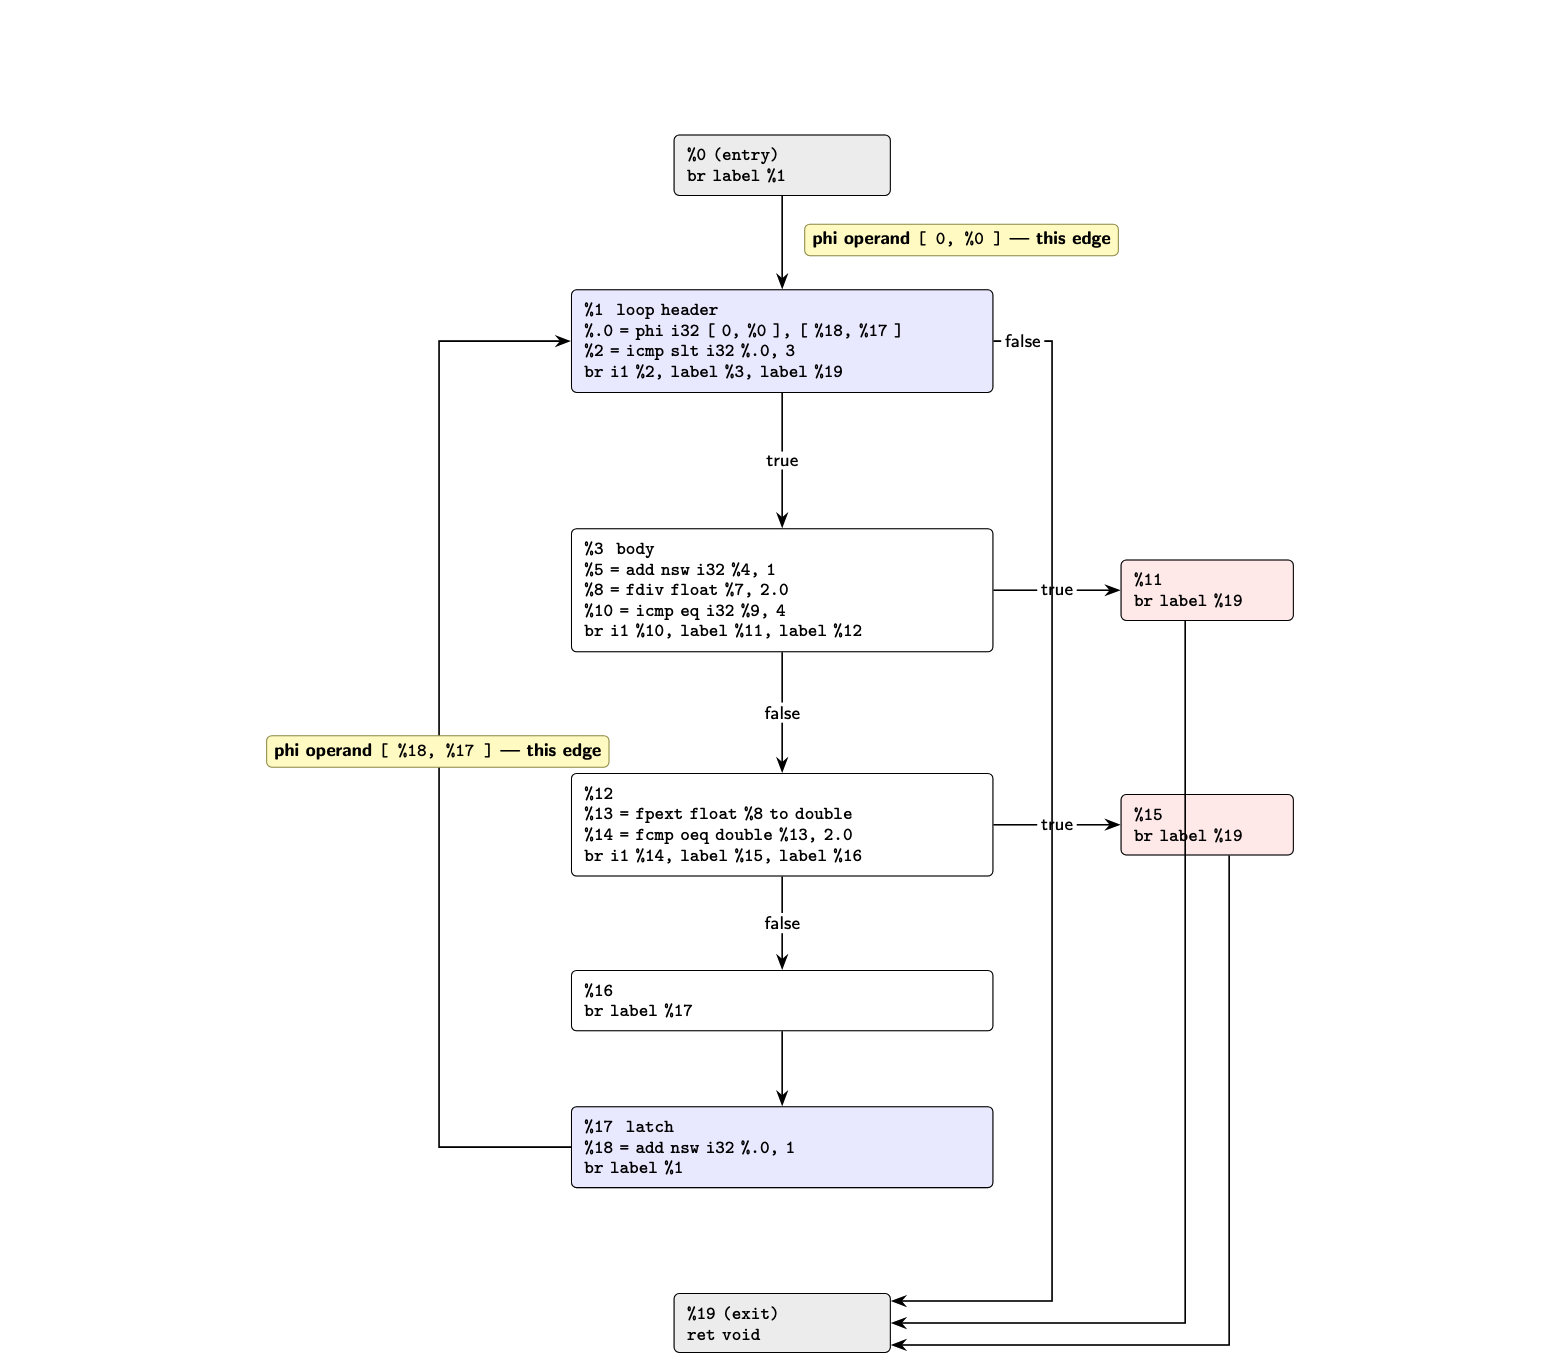
\includegraphics[width=\textwidth]{cfg.png}
  \caption{\texttt{f2} after \texttt{mem2reg} (\texttt{opt -S -passes=mem2reg opcodes.O0.ll}).}
\end{figure}


\subsection*{After \texttt{mem2reg}: struct access}

These two GEPs are from \texttt{opcodes.mem2reg.ll}
(\texttt{opt -S -passes=mem2reg opcodes.O0.ll}). After
\texttt{mem2reg}, \texttt{compiletimeindex}'s alloca is gone, so
\texttt{arr} is \texttt{\%1}.

\begin{lstlisting}
%4 = getelementptr inbounds [2 x %struct.myStruct], ptr %1, i64 0, i64 %3
%5 = getelementptr inbounds %struct.myStruct, ptr %4, i32 0, i32 0
\end{lstlisting}

The layout of \texttt{myStruct} on this target is: \texttt{scalar} at offset 0,
\texttt{array[2][2]} at bytes 4--19, 4 bytes of padding so the pointer is
aligned, \texttt{ptr} at offset 24, total size 32, alignment 8.

First GEP: \texttt{\%1} is the base of the \texttt{arr} allocation.
\texttt{i64 0} treats that pointer as pointing at one
\texttt{[2 x \%struct.myStruct]} and does not move it.
\texttt{i64 \%3} is the run-time index \texttt{runtimeindex} after
\texttt{sext}. That steps by the \emph{struct} size, so the address is
\texttt{base + 32 * runtimeindex}. Result: pointer to
\texttt{arr[runtimeindex]}.

Second GEP: the first \texttt{i32 0} is ``this struct, no extra stride''.
The second \texttt{i32 0} is field 0, which is \texttt{.scalar}. That field
is at offset \textbf{0}, not $32 \times$ anything. 32 bytes is only the
size of one \texttt{myStruct}, used by the array-element index above.

The getelementptr arithmetic is purely done on the addresses. There is no
memory access involved. The memory access is done by a separate load/store.
Hence, getelementptr does not read the memory.

\subsection*{The 2D field}

\texttt{arr[runtimeindex].array[compiletimeindex][compiletimeindex]} with
both compile-time indices equal to 0. After \texttt{mem2reg}:

\begin{lstlisting}
%8 = getelementptr inbounds [2 x %struct.myStruct], ptr %1, i64 0, i64 %7
%9 = getelementptr inbounds %struct.myStruct, ptr %8, i32 0, i32 1
%10 = getelementptr inbounds [2 x [2 x i32]], ptr %9, i64 0, i64 0
%11 = getelementptr inbounds [2 x i32], ptr %10, i64 0, i64 0
store i32 2, ptr %11, align 4
\end{lstlisting}

Same layout as above: one \texttt{myStruct} is 32 bytes, \texttt{array} starts
at byte 4, each row is 8 bytes, each \texttt{int} is 4 bytes.

\begin{tabular}{lll}
\hline
GEP & What it selects & Extra bytes \\
\hline
\texttt{i64 \%7} & \texttt{arr[runtimeindex]} & $32 \times$ \texttt{runtimeindex} \\
\texttt{i32 0, i32 1} & field 1, \texttt{.array} & $+4$ \\
\texttt{i64 0, i64 0} & row 0 of \texttt{[2][2]} & $+0$ (row 1 would be $+8$) \\
\texttt{i64 0, i64 0} & column 0 of that row & $+0$ (column 1 would be $+4$) \\
\hline
\end{tabular}

So the address is $\texttt{base} + 32\cdot\texttt{runtimeindex} + 4$.
For \texttt{runtimeindex = 1} that is 36 bytes past the start of
\texttt{arr}. The \texttt{store i32 2} is the actual write;
the GEPs only built the pointer.

\section{Part B}

Counts and named pipelines here are from Homebrew LLVM 23.1.0.

\begin{figure}[H]
  \centering
  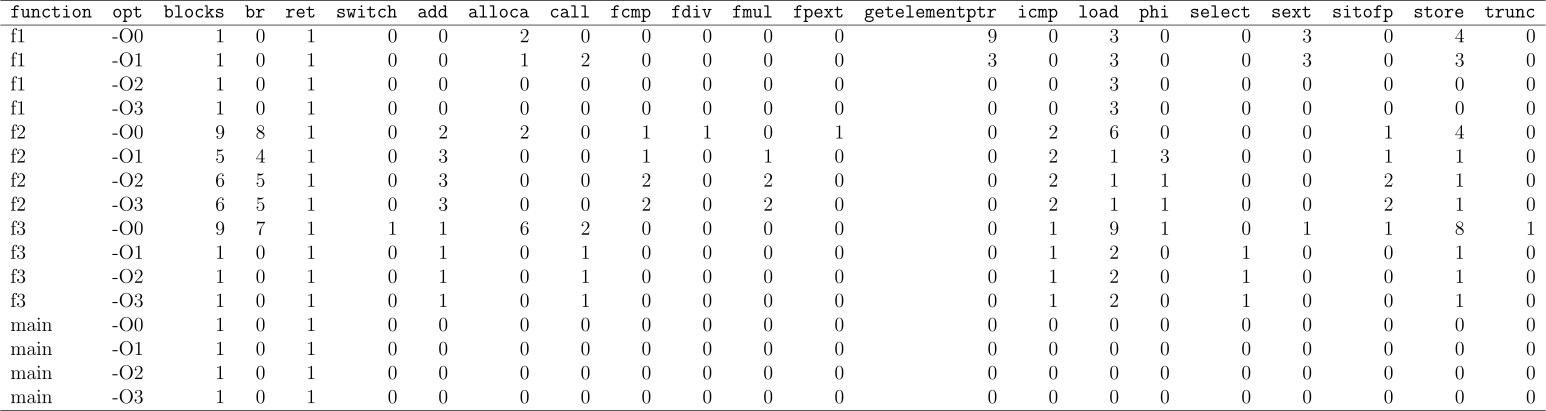
\includegraphics[width=\textwidth]{opcode_table.png}
  \caption{Opcode counts per function and optimisation level.}
\end{figure}


\subsection*{1)}

\textbf{Before:}

\begin{lstlisting}
%1 = alloca i32, align 4
store i32 0, ptr %1, align 4
br label %3

3:
%4 = load i32, ptr %1, align 4
%5 = icmp slt i32 %4, 3
br i1 %5, label %6, label %24

21:
%22 = load i32, ptr %1, align 4
%23 = add nsw i32 %22, 1
store i32 %23, ptr %1, align 4
br label %3, !llvm.loop !5
\end{lstlisting}

\textbf{After} \texttt{opt -S -passes=mem2reg opcodes.O0.ll}:

\begin{lstlisting}
br label %1

1:
%.0 = phi i32 [ 0, %0 ], [ %18, %17 ]
%2 = icmp slt i32 %.0, 3
...

17:
%18 = add nsw i32 %.0, 1
br label %1, !llvm.loop !5
\end{lstlisting}

\textbf{Explanation:} Change made by \texttt{mem2reg}. In \texttt{f2}, the loop
counter becomes a phi node. Earlier the loop counter was in the stack slot. Now
it is promoted to a register.

\subsection*{2)}

\texttt{f3} switches on \texttt{int a = 1}. At \texttt{-O0} the switch and
all four cases are still there (9 blocks, one \texttt{switch}). Cases 0, 2
and 3 are dead.

\textbf{Before} (\texttt{opcodes.O0.ll}):

\begin{lstlisting}
store i32 1, ptr %1, align 4
%6 = load i32, ptr %1, align 4
switch i32 %6, label %31 [
  i32 0, label %7
  i32 1, label %8
  i32 2, label %19
  i32 3, label %25
]
\end{lstlisting}

\textbf{After} \texttt{opt -S -passes='function(mem2reg,sccp,simplifycfg)'}:

\begin{lstlisting}
%1 = load volatile i32, ptr @runtimeindex, align 4
%2 = icmp sgt i32 %1, 1
%3 = load i32, ptr @loopcarried, align 4
%4 = select i1 %2, i32 %3, i32 7
%5 = load i32, ptr @loopcarried, align 4
%6 = add nsw i32 %5, %4
store i32 %6, ptr @loopcarried, align 4
call void @f1()
ret void
\end{lstlisting}

\texttt{sccp} sees that the switch condition is the constant 1.
\texttt{simplifycfg} deletes the unused arms and the \texttt{switch}.
What is left is only case 1: the ternary becomes a \texttt{select}, then
\texttt{call @f1}. That is why the Part B table goes from 9 blocks to 1
and from one \texttt{switch} to zero at \texttt{-O1}.

\subsection*{3)}

\textbf{Before:}

\begin{lstlisting}
3:                                                ; preds = %1
%9 = load i32, ptr @loopcarried, align 4
%10 = icmp eq i32 %9, 4
br i1 %10, label %11, label %12

11:                                               ; preds = %3
br label %19

12:                                               ; preds = %3
%13 = fpext float %8 to double
%14 = fcmp oeq double %13, 2.000000e+00
br i1 %14, label %15, label %16

15:                                               ; preds = %12
br label %19

16:                                               ; preds = %12
br label %17
\end{lstlisting}

\textbf{After:}

\begin{lstlisting}
3:                                                ; preds = %1
%9 = load i32, ptr @loopcarried, align 4
%10 = icmp eq i32 %9, 4
%11 = fpext float %8 to double
%12 = fcmp oeq double %11, 2.000000e+00
%or.cond = select i1 %10, i1 true, i1 %12
br i1 %or.cond, label %15, label %13
\end{lstlisting}

The before code is after \texttt{opt -S -passes=mem2reg opcodes.O0.ll}.
The after code is after
\texttt{opt -S -passes='mem2reg,simplifycfg' opcodes.O0.ll}.

It collapses the 2 statements in the code:

\begin{lstlisting}[language={}]
if (loopcarried == 4) break;
else if (myf == 2.0) break;
\end{lstlisting}

into a common \texttt{or.cond} check, simplifying the branch specification.

\section{Part C}

These numbers are from Homebrew LLVM 18.1.8, the same
\texttt{opt} and \texttt{clang}.

The default pipelines were printed with:

\begin{lstlisting}[language={},basicstyle=\ttfamily\footnotesize]
opt -passes="default<O1>" -print-pipeline-passes -disable-output opcodes.O0.ll
\end{lstlisting}

The same command was run for \texttt{O0}, \texttt{O2} and \texttt{O3}.
\texttt{opt --print-passes} was used to see which names are real
transforms and which are only analyses.

The dump is not only transforms. It also wraps passes in
\texttt{function} and \texttt{loop}, and it prints analyses such as
\texttt{require}, \texttt{invalidate} and \texttt{verify}. Those were
left out of the count. There is also an AArch64 class name that
\texttt{opt} will not take as a pass, so that was left out too. If
the same transform ran more than once each run was kept in the
order it appeared.

\subsection*{Counts}

\begin{tabular}{lrr}
\hline
Level & Invocations & Distinct \\
\hline
\texttt{-O0} & 5 & 5 \\
\texttt{-O1} & 81 & 55 \\
\texttt{-O2} & 97 & 66 \\
\texttt{-O3} & 100 & 69 \\
\hline
\end{tabular}

\subsection*{Ordered lists}

Passes in the order they ran.

{\fontsize{5.4pt}{6.6pt}\selectfont
\setlength{\tabcolsep}{5pt}
\renewcommand{\arraystretch}{1.15}
\begin{longtable}{llll}
\hline
\texttt{-O0} & \texttt{-O1} & \texttt{-O2} & \texttt{-O3} \\
\hline
\endfirsthead
\hline
\texttt{-O0} & \texttt{-O1} & \texttt{-O2} & \texttt{-O3} \\
\hline
\endhead
1.~\texttt{always-inline} & 1.~\texttt{annotation2metadata} & 1.~\texttt{annotation2metadata} & 1.~\texttt{annotation2metadata} \\
2.~\texttt{coro-early} & 2.~\texttt{forceattrs} & 2.~\texttt{forceattrs} & 2.~\texttt{forceattrs} \\
3.~\texttt{coro-split} & 3.~\texttt{inferattrs} & 3.~\texttt{inferattrs} & 3.~\texttt{inferattrs} \\
4.~\texttt{coro-cleanup} & 4.~\texttt{coro-early} & 4.~\texttt{coro-early} & 4.~\texttt{coro-early} \\
5.~\texttt{globaldce} & 5.~\texttt{lower-expect} & 5.~\texttt{lower-expect} & 5.~\texttt{lower-expect} \\
 & 6.~\texttt{simplifycfg} & 6.~\texttt{simplifycfg} & 6.~\texttt{simplifycfg} \\
 & 7.~\texttt{sroa} & 7.~\texttt{sroa} & 7.~\texttt{sroa} \\
 & 8.~\texttt{early-cse} & 8.~\texttt{early-cse} & 8.~\texttt{early-cse} \\
 & 9.~\texttt{openmp-opt} & 9.~\texttt{openmp-opt} & 9.~\texttt{callsite-splitting} \\
 & 10.~\texttt{ipsccp} & 10.~\texttt{ipsccp} & 10.~\texttt{openmp-opt} \\
 & 11.~\texttt{called-value-propagation} & 11.~\texttt{called-value-propagation} & 11.~\texttt{ipsccp} \\
 & 12.~\texttt{globalopt} & 12.~\texttt{globalopt} & 12.~\texttt{called-value-propagation} \\
 & 13.~\texttt{mem2reg} & 13.~\texttt{mem2reg} & 13.~\texttt{globalopt} \\
 & 14.~\texttt{instcombine} & 14.~\texttt{instcombine} & 14.~\texttt{mem2reg} \\
 & 15.~\texttt{simplifycfg} & 15.~\texttt{simplifycfg} & 15.~\texttt{instcombine} \\
 & 16.~\texttt{always-inline} & 16.~\texttt{always-inline} & 16.~\texttt{simplifycfg} \\
 & 17.~\texttt{inline} & 17.~\texttt{inline} & 17.~\texttt{always-inline} \\
 & 18.~\texttt{function-attrs} & 18.~\texttt{function-attrs} & 18.~\texttt{inline} \\
 & 19.~\texttt{sroa} & 19.~\texttt{openmp-opt-cgscc} & 19.~\texttt{function-attrs} \\
 & 20.~\texttt{early-cse} & 20.~\texttt{sroa} & 20.~\texttt{argpromotion} \\
 & 21.~\texttt{simplifycfg} & 21.~\texttt{early-cse} & 21.~\texttt{openmp-opt-cgscc} \\
 & 22.~\texttt{instcombine} & 22.~\texttt{speculative-execution} & 22.~\texttt{sroa} \\
 & 23.~\texttt{libcalls-shrinkwrap} & 23.~\texttt{jump-threading} & 23.~\texttt{early-cse} \\
 & 24.~\texttt{simplifycfg} & 24.~\texttt{correlated-propagation} & 24.~\texttt{speculative-execution} \\
 & 25.~\texttt{reassociate} & 25.~\texttt{simplifycfg} & 25.~\texttt{jump-threading} \\
 & 26.~\texttt{loop-instsimplify} & 26.~\texttt{instcombine} & 26.~\texttt{correlated-propagation} \\
 & 27.~\texttt{loop-simplifycfg} & 27.~\texttt{aggressive-instcombine} & 27.~\texttt{simplifycfg} \\
 & 28.~\texttt{licm} & 28.~\texttt{libcalls-shrinkwrap} & 28.~\texttt{instcombine} \\
 & 29.~\texttt{loop-rotate} & 29.~\texttt{tailcallelim} & 29.~\texttt{aggressive-instcombine} \\
 & 30.~\texttt{licm} & 30.~\texttt{simplifycfg} & 30.~\texttt{libcalls-shrinkwrap} \\
 & 31.~\texttt{simple-loop-unswitch} & 31.~\texttt{reassociate} & 31.~\texttt{tailcallelim} \\
 & 32.~\texttt{simplifycfg} & 32.~\texttt{constraint-elimination} & 32.~\texttt{simplifycfg} \\
 & 33.~\texttt{instcombine} & 33.~\texttt{loop-instsimplify} & 33.~\texttt{reassociate} \\
 & 34.~\texttt{loop-idiom} & 34.~\texttt{loop-simplifycfg} & 34.~\texttt{constraint-elimination} \\
 & 35.~\texttt{indvars} & 35.~\texttt{licm} & 35.~\texttt{loop-instsimplify} \\
 & 36.~\texttt{loop-deletion} & 36.~\texttt{loop-rotate} & 36.~\texttt{loop-simplifycfg} \\
 & 37.~\texttt{loop-unroll-full} & 37.~\texttt{licm} & 37.~\texttt{licm} \\
 & 38.~\texttt{sroa} & 38.~\texttt{simple-loop-unswitch} & 38.~\texttt{loop-rotate} \\
 & 39.~\texttt{memcpyopt} & 39.~\texttt{simplifycfg} & 39.~\texttt{licm} \\
 & 40.~\texttt{sccp} & 40.~\texttt{instcombine} & 40.~\texttt{simple-loop-unswitch} \\
 & 41.~\texttt{bdce} & 41.~\texttt{loop-idiom} & 41.~\texttt{simplifycfg} \\
 & 42.~\texttt{instcombine} & 42.~\texttt{indvars} & 42.~\texttt{instcombine} \\
 & 43.~\texttt{coro-elide} & 43.~\texttt{loop-deletion} & 43.~\texttt{loop-idiom} \\
 & 44.~\texttt{adce} & 44.~\texttt{loop-unroll-full} & 44.~\texttt{indvars} \\
 & 45.~\texttt{simplifycfg} & 45.~\texttt{sroa} & 45.~\texttt{loop-deletion} \\
 & 46.~\texttt{instcombine} & 46.~\texttt{vector-combine} & 46.~\texttt{loop-unroll-full} \\
 & 47.~\texttt{function-attrs} & 47.~\texttt{mldst-motion} & 47.~\texttt{sroa} \\
 & 48.~\texttt{coro-split} & 48.~\texttt{gvn} & 48.~\texttt{vector-combine} \\
 & 49.~\texttt{deadargelim} & 49.~\texttt{sccp} & 49.~\texttt{mldst-motion} \\
 & 50.~\texttt{coro-cleanup} & 50.~\texttt{bdce} & 50.~\texttt{gvn} \\
 & 51.~\texttt{globalopt} & 51.~\texttt{instcombine} & 51.~\texttt{sccp} \\
 & 52.~\texttt{globaldce} & 52.~\texttt{jump-threading} & 52.~\texttt{bdce} \\
 & 53.~\texttt{elim-avail-extern} & 53.~\texttt{correlated-propagation} & 53.~\texttt{instcombine} \\
 & 54.~\texttt{rpo-function-attrs} & 54.~\texttt{adce} & 54.~\texttt{jump-threading} \\
 & 55.~\texttt{float2int} & 55.~\texttt{memcpyopt} & 55.~\texttt{correlated-propagation} \\
 & 56.~\texttt{lower-constant-intrinsics} & 56.~\texttt{dse} & 56.~\texttt{adce} \\
 & 57.~\texttt{loop-rotate} & 57.~\texttt{move-auto-init} & 57.~\texttt{memcpyopt} \\
 & 58.~\texttt{loop-deletion} & 58.~\texttt{licm} & 58.~\texttt{dse} \\
 & 59.~\texttt{loop-distribute} & 59.~\texttt{coro-elide} & 59.~\texttt{move-auto-init} \\
 & 60.~\texttt{inject-tli-mappings} & 60.~\texttt{simplifycfg} & 60.~\texttt{licm} \\
 & 61.~\texttt{loop-vectorize} & 61.~\texttt{instcombine} & 61.~\texttt{coro-elide} \\
 & 62.~\texttt{infer-alignment} & 62.~\texttt{function-attrs} & 62.~\texttt{simplifycfg} \\
 & 63.~\texttt{loop-load-elim} & 63.~\texttt{coro-split} & 63.~\texttt{instcombine} \\
 & 64.~\texttt{instcombine} & 64.~\texttt{deadargelim} & 64.~\texttt{function-attrs} \\
 & 65.~\texttt{simplifycfg} & 65.~\texttt{coro-cleanup} & 65.~\texttt{coro-split} \\
 & 66.~\texttt{vector-combine} & 66.~\texttt{globalopt} & 66.~\texttt{deadargelim} \\
 & 67.~\texttt{instcombine} & 67.~\texttt{globaldce} & 67.~\texttt{coro-cleanup} \\
 & 68.~\texttt{loop-unroll} & 68.~\texttt{elim-avail-extern} & 68.~\texttt{globalopt} \\
 & 69.~\texttt{sroa} & 69.~\texttt{rpo-function-attrs} & 69.~\texttt{globaldce} \\
 & 70.~\texttt{infer-alignment} & 70.~\texttt{float2int} & 70.~\texttt{elim-avail-extern} \\
 & 71.~\texttt{instcombine} & 71.~\texttt{lower-constant-intrinsics} & 71.~\texttt{rpo-function-attrs} \\
 & 72.~\texttt{licm} & 72.~\texttt{loop-rotate} & 72.~\texttt{float2int} \\
 & 73.~\texttt{alignment-from-assumptions} & 73.~\texttt{loop-deletion} & 73.~\texttt{lower-constant-intrinsics} \\
 & 74.~\texttt{loop-sink} & 74.~\texttt{loop-distribute} & 74.~\texttt{chr} \\
 & 75.~\texttt{instsimplify} & 75.~\texttt{inject-tli-mappings} & 75.~\texttt{loop-rotate} \\
 & 76.~\texttt{div-rem-pairs} & 76.~\texttt{loop-vectorize} & 76.~\texttt{loop-deletion} \\
 & 77.~\texttt{tailcallelim} & 77.~\texttt{infer-alignment} & 77.~\texttt{loop-distribute} \\
 & 78.~\texttt{simplifycfg} & 78.~\texttt{loop-load-elim} & 78.~\texttt{inject-tli-mappings} \\
 & 79.~\texttt{globaldce} & 79.~\texttt{instcombine} & 79.~\texttt{loop-vectorize} \\
 & 80.~\texttt{constmerge} & 80.~\texttt{simplifycfg} & 80.~\texttt{infer-alignment} \\
 & 81.~\texttt{rel-lookup-table-converter} & 81.~\texttt{slp-vectorizer} & 81.~\texttt{loop-load-elim} \\
 &  & 82.~\texttt{vector-combine} & 82.~\texttt{instcombine} \\
 &  & 83.~\texttt{instcombine} & 83.~\texttt{simplifycfg} \\
 &  & 84.~\texttt{loop-unroll} & 84.~\texttt{slp-vectorizer} \\
 &  & 85.~\texttt{sroa} & 85.~\texttt{vector-combine} \\
 &  & 86.~\texttt{infer-alignment} & 86.~\texttt{instcombine} \\
 &  & 87.~\texttt{instcombine} & 87.~\texttt{loop-unroll} \\
 &  & 88.~\texttt{licm} & 88.~\texttt{sroa} \\
 &  & 89.~\texttt{alignment-from-assumptions} & 89.~\texttt{infer-alignment} \\
 &  & 90.~\texttt{loop-sink} & 90.~\texttt{instcombine} \\
 &  & 91.~\texttt{instsimplify} & 91.~\texttt{licm} \\
 &  & 92.~\texttt{div-rem-pairs} & 92.~\texttt{alignment-from-assumptions} \\
 &  & 93.~\texttt{tailcallelim} & 93.~\texttt{loop-sink} \\
 &  & 94.~\texttt{simplifycfg} & 94.~\texttt{instsimplify} \\
 &  & 95.~\texttt{globaldce} & 95.~\texttt{div-rem-pairs} \\
 &  & 96.~\texttt{constmerge} & 96.~\texttt{tailcallelim} \\
 &  & 97.~\texttt{rel-lookup-table-converter} & 97.~\texttt{simplifycfg} \\
 &  &  & 98.~\texttt{globaldce} \\
 &  &  & 99.~\texttt{constmerge} \\
 &  &  & 100.~\texttt{rel-lookup-table-converter} \\
\hline
\end{longtable}
}

\subsection*{Pass descriptions}

{\small
\begin{longtable}{lp{6.4cm}rrrr}
\hline
Pass & Description & \texttt{-O0} & \texttt{-O1} & \texttt{-O2} & \texttt{-O3} \\
\hline
\endfirsthead
\hline
Pass & Description & \texttt{-O0} & \texttt{-O1} & \texttt{-O2} & \texttt{-O3} \\
\hline
\endhead
\texttt{adce} & Removes instructions whose results are never used. & 0 & 1 & 1 & 1 \\
\texttt{aggressive-instcombine} & Extra peephole simplifications, only worth running from \texttt{-O2}. & 0 & 0 & 1 & 1 \\
\texttt{alignment-from-assumptions} & Improves load/store alignment using \texttt{llvm.assume} hints. & 0 & 1 & 1 & 1 \\
\texttt{always-inline} & Inlines functions marked \texttt{always\_inline}. & 1 & 1 & 1 & 1 \\
\texttt{annotation2metadata} & Turns source annotations into IR metadata. & 0 & 1 & 1 & 1 \\
\texttt{argpromotion} & Replaces a read-only pointer argument with its value. & 0 & 0 & 0 & 1 \\
\texttt{bdce} & Removes individually unused bits of a value. & 0 & 1 & 1 & 1 \\
\texttt{called-value-propagation} & Figures out the target of an indirect call when possible. & 0 & 1 & 1 & 1 \\
\texttt{callsite-splitting} & Splits a call so each caller path can be optimised separately. & 0 & 0 & 0 & 1 \\
\texttt{chr} & Straightens out a chain of hot/cold branches. & 0 & 0 & 0 & 1 \\
\texttt{constmerge} & Merges multiple global constants that have identical values into one. & 0 & 1 & 1 & 1 \\
\texttt{constraint-elimination} & Removes comparisons already implied by an earlier one. & 0 & 0 & 1 & 1 \\
\texttt{coro-cleanup} & Final cleanup step for coroutines. & 1 & 1 & 1 & 1 \\
\texttt{coro-early} & Early setup step for coroutines. & 1 & 1 & 1 & 1 \\
\texttt{coro-elide} & Skips allocating a coroutine frame when not needed. & 0 & 1 & 1 & 1 \\
\texttt{coro-split} & Splits a coroutine into its resume/destroy/cleanup parts. & 1 & 1 & 1 & 1 \\
\texttt{correlated-propagation} & Reuses facts proven true earlier in a branch. & 0 & 0 & 2 & 2 \\
\texttt{deadargelim} & Removes unused function arguments. & 0 & 1 & 1 & 1 \\
\texttt{div-rem-pairs} & Keeps a matching div and rem together for one instruction. & 0 & 1 & 1 & 1 \\
\texttt{dse} & Removes a store that gets overwritten before it's read. & 0 & 0 & 1 & 1 \\
\texttt{early-cse} & Removes duplicate computations early, before loop passes run. & 0 & 2 & 2 & 2 \\
\texttt{elim-avail-extern} & Drops function bodies that are no longer needed locally. & 0 & 1 & 1 & 1 \\
\texttt{float2int} & Does float work as integers when the result is the same. & 0 & 1 & 1 & 1 \\
\texttt{forceattrs} & Applies attributes passed on the command line. & 0 & 1 & 1 & 1 \\
\texttt{function-attrs} & Marks functions as \texttt{readonly}, \texttt{nocapture}, and similar. & 0 & 2 & 2 & 2 \\
\texttt{globaldce} & Removes globals and functions that are never used. & 1 & 2 & 2 & 2 \\
\texttt{globalopt} & Simplifies and shrinks global variables. & 0 & 2 & 2 & 2 \\
\texttt{gvn} & Removes a computation that duplicates an earlier one. & 0 & 0 & 1 & 1 \\
\texttt{indvars} & Simplifies loop counters into a standard form. & 0 & 1 & 1 & 1 \\
\texttt{infer-alignment} & Works out stronger alignment for loads and stores. & 0 & 2 & 2 & 2 \\
\texttt{inferattrs} & Adds known attributes to standard library calls. & 0 & 1 & 1 & 1 \\
\texttt{inject-tli-mappings} & Notes which library calls have a vector version. & 0 & 1 & 1 & 1 \\
\texttt{inline} & The main inliner, based on a cost heuristic. & 0 & 1 & 1 & 1 \\
\texttt{instcombine} & General peephole simplifier; runs many times. & 0 & 8 & 8 & 8 \\
\texttt{instsimplify} & Simplifies instructions without creating new ones. & 0 & 1 & 1 & 1 \\
\texttt{ipsccp} & Propagates constants across function calls. & 0 & 1 & 1 & 1 \\
\texttt{jump-threading} & Skips a branch whose outcome is already known. & 0 & 0 & 2 & 2 \\
\texttt{libcalls-shrinkwrap} & Guards an expensive library call with a cheap check. & 0 & 1 & 1 & 1 \\
\texttt{licm} & Moves loop-invariant work out of the loop. & 0 & 3 & 4 & 4 \\
\texttt{loop-deletion} & Removes loops that have no effect. & 0 & 2 & 2 & 2 \\
\texttt{loop-distribute} & Splits one loop into two independent loops. & 0 & 1 & 1 & 1 \\
\texttt{loop-idiom} & Replaces a copy-style loop with \texttt{memcpy}. & 0 & 1 & 1 & 1 \\
\texttt{loop-instsimplify} & Runs instruction simplification inside loops. & 0 & 1 & 1 & 1 \\
\texttt{loop-load-elim} & Avoids reloading a value already stored last iteration. & 0 & 1 & 1 & 1 \\
\texttt{loop-rotate} & Turns a while-style loop into a do-while-style loop. & 0 & 2 & 2 & 2 \\
\texttt{loop-simplifycfg} & Simplifies the control flow inside a loop. & 0 & 1 & 1 & 1 \\
\texttt{loop-sink} & Moves work into the part of the loop that needs it. & 0 & 1 & 1 & 1 \\
\texttt{loop-unroll} & Unrolls a loop a few times. & 0 & 1 & 1 & 1 \\
\texttt{loop-unroll-full} & Fully unrolls a loop with a small constant trip count. & 0 & 1 & 1 & 1 \\
\texttt{loop-vectorize} & Rewrites a loop to use vector instructions. & 0 & 1 & 1 & 1 \\
\texttt{lower-constant-intrinsics} & Expands intrinsics like \texttt{llvm.objectsize} into constants. & 0 & 1 & 1 & 1 \\
\texttt{lower-expect} & Turns \texttt{llvm.expect} hints into branch weights. & 0 & 1 & 1 & 1 \\
\texttt{mem2reg} & Promotes stack slots into SSA registers. & 0 & 1 & 1 & 1 \\
\texttt{memcpyopt} & Replaces copy-style load/store sequences with \texttt{memcpy}. & 0 & 1 & 1 & 1 \\
\texttt{mldst-motion} & Hoists a load/store shared by both if/else branches. & 0 & 0 & 1 & 1 \\
\texttt{move-auto-init} & Moves variable-init memsets off the hot path. & 0 & 0 & 1 & 1 \\
\texttt{openmp-opt} & Optimises OpenMP calls (not used here). & 0 & 1 & 1 & 1 \\
\texttt{openmp-opt-cgscc} & OpenMP optimisation run alongside the inliner. & 0 & 0 & 1 & 1 \\
\texttt{reassociate} & Reorders \texttt{+}/\texttt{*} chains to expose more folding. & 0 & 1 & 1 & 1 \\
\texttt{rel-lookup-table-converter} & Makes switch jump tables use relative offsets. & 0 & 1 & 1 & 1 \\
\texttt{rpo-function-attrs} & Infers function attributes across the call graph. & 0 & 1 & 1 & 1 \\
\texttt{sccp} & Folds a value to a constant along reachable branches only. & 0 & 1 & 1 & 1 \\
\texttt{simple-loop-unswitch} & Pulls a loop-invariant branch out of the loop. & 0 & 1 & 1 & 1 \\
\texttt{simplifycfg} & Fewer blocks and branches; runs many times. & 0 & 8 & 8 & 8 \\
\texttt{slp-vectorizer} & Vectorises independent scalar ops within one block. & 0 & 0 & 1 & 1 \\
\texttt{speculative-execution} & Hoists a cheap op above a branch when safe. & 0 & 0 & 1 & 1 \\
\texttt{sroa} & Breaks a struct/array alloca into separate scalars. & 0 & 4 & 4 & 4 \\
\texttt{tailcallelim} & Turns a tail call into a jump back to the start. & 0 & 1 & 2 & 2 \\
\texttt{vector-combine} & Cleans up vector instructions after vectorisation. & 0 & 1 & 2 & 2 \\
\hline
\end{longtable}
}

\subsection*{1)}

\textbf{i) transformations common to all four levels:}

Only these five names appear at \texttt{-O0}, \texttt{-O1},
\texttt{-O2} and \texttt{-O3}. \texttt{-O0} is just always-inline, the
coroutine lowering, and a global DCE. Nothing like mem2reg or
instcombine runs there.

\begin{lstlisting}[language={}]
always-inline, coro-early, coro-split, coro-cleanup, globaldce
\end{lstlisting}

\subsection*{2)}

\textbf{ii) transformations first introduced at O1, O2, or O3:}

First introduced at \texttt{-O1}. This is where the real pipeline
starts. The rest of the O1 ordered list above is also new here; it
is just not repeated in the box.

\begin{lstlisting}[language={}]
mem2reg, sroa, instcombine, simplifycfg, inline, ipsccp,
licm, loop-rotate, indvars, loop-unroll, loop-vectorize,
sccp, adce
\end{lstlisting}

First introduced at \texttt{-O2}. Extra jump cleanup, redundancy
elimination, SLP vectorisation, and a few CGSCC passes.

\begin{lstlisting}[language={}]
jump-threading, correlated-propagation, gvn, dse,
slp-vectorizer, aggressive-instcombine, constraint-elimination,
mldst-motion, speculative-execution, move-auto-init,
openmp-opt-cgscc
\end{lstlisting}

First introduced at \texttt{-O3}. Only three new names.

\begin{lstlisting}[language={}]
callsite-splitting, argpromotion, chr
\end{lstlisting}

\subsection*{3)}

\textbf{iii) transformations whose number or position of invocations
changes between levels:}

Most names that appear at \texttt{-O1} keep the same count at
\texttt{-O2} and \texttt{-O3}. A few do not: they either run more
often, or they already run more than once the first time they
appear. The table is how many times each of those names showed up
in our dump.

{\small
\begin{tabular}{lcccc}
\hline
Pass & \texttt{-O0} & \texttt{-O1} & \texttt{-O2} & \texttt{-O3} \\
\hline
\texttt{globaldce} & 1 & 2 & 2 & 2 \\
\texttt{licm} & 0 & 3 & 4 & 4 \\
\texttt{tailcallelim} & 0 & 1 & 2 & 2 \\
\texttt{vector-combine} & 0 & 1 & 2 & 2 \\
\texttt{jump-threading} & 0 & 0 & 2 & 2 \\
\texttt{correlated-propagation} & 0 & 0 & 2 & 2 \\
\texttt{instcombine} & 0 & 8 & 8 & 8 \\
\texttt{simplifycfg} & 0 & 8 & 8 & 8 \\
\hline
\end{tabular}
}

\texttt{globaldce} already runs at \texttt{-O0}. From \texttt{-O1} it
runs twice: once after coroutine cleanup, and once near the end.

\texttt{licm} is 3 times at \texttt{-O1} and 4 times from
\texttt{-O2}, because O2 adds one more licm after dse.

\texttt{tailcallelim} is once at the end of O1. From O2 it also
runs earlier, in the CGSCC block after the inliner.

\texttt{vector-combine} is once at O1. From O2 it runs after the
mid-pipeline sroa, and again after slp-vectorizer.

\texttt{jump-threading} and \texttt{correlated-propagation} are not
in O1 at all. When they start at O2 they already run twice: once
before the loop nest and once after it.

\texttt{instcombine} and \texttt{simplifycfg} still run 8 times
from O1 onwards. Other passes keep making new work for them, so they
are run again and how often they run does not change. Where they sit
in the list does because O2 and O3 put extra passes in between.

Those extra passes also slide most O1 names further down the
list. The first five stay put, that is slots 1 to 5 are still
\texttt{annotation2metadata}, \texttt{forceattrs},
\texttt{inferattrs}, \texttt{coro-early} and
\texttt{lower-expect}. After that the numbers move. 
{\small
\begin{tabular}{lccc}
\hline
Pass & \texttt{-O1} slots & \texttt{-O2} slots & \texttt{-O3} slots \\
\hline
\texttt{mem2reg} & 13 & 13 & 14 \\
\texttt{memcpyopt} & 39 & 55 & 57 \\
\texttt{loop-vectorize} & 61 & 76 & 79 \\
\texttt{loop-unroll} & 68 & 84 & 87 \\
\hline
\end{tabular}
}

\texttt{instcombine} also moves, but it has eight places at each
level, so that is a separate table:

{\small
\begin{tabular}{ll}
\hline
Level & Slots \\
\hline
\texttt{-O1} & 14, 22, 33, 42, 46, 64, 67, 71 \\
\texttt{-O2} & 14, 26, 40, 51, 61, 79, 83, 87 \\
\texttt{-O3} & 15, 28, 42, 53, 63, 82, 86, 90 \\
\hline
\end{tabular}
}

\texttt{memcpyopt} is easy to see. At O1 it is right after the
\texttt{sroa} that follows \texttt{loop-unroll-full} (slot 38, then
39). At O2 it comes after \texttt{adce}, because \texttt{gvn} and
\texttt{jump-threading} run first.

The same name can also be given different options.

\begin{lstlisting}[language={}]
loop-unroll, loop-vectorize, simple-loop-unswitch
\end{lstlisting}

\texttt{loop-unroll} is printed as \texttt{loop-unroll<O1>},
\texttt{loop-unroll<O2>} or \texttt{loop-unroll<O3>}. A higher
level unrolls more.

\texttt{loop-vectorize} at O1 is marked
\texttt{vectorize-forced-only}. At O2 and O3 that flag is off, so
the loop is actually vectorised from O2.

\texttt{simple-loop-unswitch} at O1 and O2 only does the cheap
(trivial) case. At O3 it is
\texttt{<nontrivial;trivial>}, so it also tries the harder case.

\section{Part D}

\texttt{f1}, \texttt{f2} and \texttt{f3} are the three required loops
in \texttt{vector.c}. \texttt{f4} is a small extra interleave so that
\texttt{shufflevector} shows up. Length is an argument. Array pointers
that must not overlap are \texttt{restrict}. \texttt{main} uses buffers
of 4096 elements and prints a checksum for five sizes.

Scalar IR first, then native vector IR (Homebrew LLVM 18.1.8).
\texttt{-march=native} here means NEON, not AVX.

\begin{lstlisting}[language={},basicstyle=\ttfamily\footnotesize]
clang -O3 -fno-vectorize -fno-slp-vectorize -S -emit-llvm vector.c -o vector.scalar.ll
\end{lstlisting}

\begin{lstlisting}[language={},basicstyle=\ttfamily\footnotesize]
clang -O3 -march=native -Rpass=loop-vectorize -Rpass-missed=loop-vectorize \
  -Rpass-analysis=loop-vectorize -S -emit-llvm vector.c -o vector.vector.ll \
  2> vector.remarks.txt
\end{lstlisting}

With vectorisation off, each step is one scalar load / arithmetic /
store. The remarks with it on are:

\begin{lstlisting}[language={}]
vector.c:8:  vectorized loop (vectorization width: 4, interleaved count: 4)
vector.c:16: vectorized loop (vectorization width: 4, interleaved count: 4)
vector.c:24: vectorized loop (vectorization width: 4, interleaved count: 4)
vector.c:33: vectorized loop (vectorization width: 4, interleaved count: 2)
\end{lstlisting}

{\small
\begin{tabular}{llll}
\hline
Loop & What it does & Width & Interleave \\
\hline
\texttt{f1} & float $a[i]\times\texttt{alph}+b[i]$ & 4 & 4 \\
\texttt{f2} & integer dot product & 4 & 4 \\
\texttt{f3} & pick $a[i]$ or $b[i]$ from \texttt{guess} & 4 & 4 \\
\texttt{f4} & write $a[i]$, $b[i]$ into even/odd slots & 4 & 2 \\
\hline
\end{tabular}
}

Width 4 is 128-bit NEON divided by a 32-bit \texttt{float} or
\texttt{i32}. Interleave 4 means four of those vectors in the body, so
16 source iterations per trip of \texttt{f1}--\texttt{f3}. The leftover
tail is scalar, which is why $n=7$ still works.

The vector types in \texttt{vector.vector.ll} are \texttt{<4 x float>},
\texttt{<4 x i32>}, \texttt{<4 x i1>} and \texttt{<8 x i32>}.

\subsection*{Tracing \texttt{f3}}

This is the load / compare / select / store walk. The C is
\texttt{c[i] = guess[i] ? a\_val : b\_val} after both ints are loaded.
One of the four interleaved steps looks like:

\begin{lstlisting}
%18 = load <4 x i32>, ptr %14
%26 = load <4 x i32>, ptr %22
%34 = load <4 x i32>, ptr %30
%38 = icmp eq <4 x i32> %34, zeroinitializer
%42 = select <4 x i1> %38, <4 x i32> %26, <4 x i32> %18
store <4 x i32> %42, ptr %46
\end{lstlisting}

\texttt{\%18} is four \texttt{a[i]}, \texttt{\%26} is four
\texttt{b[i]}, \texttt{\%34} is four \texttt{guess[i]}.
\texttt{icmp eq} against zero makes a \texttt{<4 x i1>} mask.
\texttt{select} takes \texttt{b} when \texttt{guess} is 0, else
\texttt{a}. Then four \texttt{c[i]} values are stored.

\subsection*{When \texttt{f3} did not vectorise}

The first body selected pointers, not values:

\begin{lstlisting}[language={}]
for (int i = 0; i < n; i++)
  c[i] = guess[i] ? a[i] : b[i];
\end{lstlisting}

\texttt{-Rpass-missed=loop-vectorize} printed nothing for this loop.
The cost-model note only shows up with
\texttt{-Rpass-analysis=loop-vectorize}. What clang did print:

\begin{lstlisting}[language={}]
vector.c: remark: the cost-model indicates that vectorization is not beneficial [-Rpass-analysis=loop-vectorize]
vector.c: remark: interleaved loop (interleaved count: 4) [-Rpass=loop-vectorize]
\end{lstlisting}

The IR then selected an \texttt{a} or \texttt{b} pointer
(\texttt{select i1 ..., ptr ..., ptr ...}) and did a scalar load.
There was no \texttt{<4 x i32> select}. An \texttt{if}/\texttt{else}
that wrote \texttt{c[i]} got the same two remarks.

Only the loop body was changed. Loading both ints first, then using
\texttt{?:} on the values, is the form that vectorises:

\begin{lstlisting}[language={}]
for (int i = 0; i < n; i++) {
  int a_val = a[i];
  int b_val = b[i];
  c[i] = guess[i] ? a_val : b_val;
}
\end{lstlisting}

That is the version in \texttt{vector.c} now, and the trace above.

\subsection*{\texttt{f1}: splat and FMA}

\texttt{alph} is one scalar, so it is copied into every lane of a
\texttt{<4 x float>} before the loop:

\begin{lstlisting}
%12 = insertelement <4 x float> poison, float %4, i64 0
%13 = shufflevector <4 x float> %12, <4 x float> poison,
                    <4 x i32> zeroinitializer
\end{lstlisting}

\texttt{insertelement} puts \texttt{alph} in lane 0. The shuffle mask
is all zeros, so every lane becomes that same value.

Then each step is load / fused multiply-add / store:

\begin{lstlisting}
%20 = load <4 x float>, ptr %16
%28 = load <4 x float>, ptr %24
%32 = call <4 x float> @llvm.fmuladd.v4f32(
        <4 x float> %20, <4 x float> %13, <4 x float> %28)
store <4 x float> %32, ptr %36
\end{lstlisting}

Four \texttt{a[i]}, four \texttt{b[i]}, the broadcast \texttt{alph},
four \texttt{c[i]} stored together. There are four copies of this
because the interleave count is 4.

\subsection*{\texttt{f2}: integer reduction}

\texttt{dot += a[i] * b[i]}. The loop keeps four \texttt{<4 x i32>}
partial sums (the interleave). After the loop they are added and
folded with:

\begin{lstlisting}
%46 = call i32 @llvm.vector.reduce.add.v4i32(<4 x i32> %45)
\end{lstlisting}

That intrinsic is the horizontal add. There is no
\texttt{extractelement}. Any leftover iterations use a scalar
\texttt{phi}, same as the no-vectorise file.

\subsection*{Vector-specific opcodes}

\textbf{\texttt{insertelement}.} Only the \texttt{alph} splat in
\texttt{f1}.

\textbf{\texttt{shufflevector}.} The all-zero mask above is the
broadcast. The other use is \texttt{f4}
(\texttt{c[2*i]=a[i]; c[2*i+1]=b[i];}):

\begin{lstlisting}
%29 = shufflevector <4 x i32> %17, <4 x i32> %23,
     <8 x i32> <i32 0, i32 4, i32 1, i32 5,
                i32 2, i32 6, i32 3, i32 7>
store <8 x i32> %29, ptr %27
\end{lstlisting}

The mask \texttt{0,4,1,5,\ldots} is \texttt{a0,b0,a1,b1,\ldots}. The
result is \texttt{<8 x i32>}, so eight ints go out in one store.
Interleave 2 means two of these shuffles per trip.

\textbf{\texttt{extractelement}.} Not emitted. The reduction uses
\texttt{llvm.vector.reduce.add.v4i32} instead of pulling lanes out.
\texttt{f4} was added for a real shuffle; it still did not produce
\texttt{extractelement}.

\textbf{\texttt{select}.} The vector \texttt{select <4 x i1>} in
\texttt{f3}.

\subsection*{Correctness}

\begin{lstlisting}[language={},basicstyle=\ttfamily\footnotesize]
clang -O3 -fno-vectorize -fno-slp-vectorize vector.c -o vector.scalar
clang -O3 -march=native vector.c -o vector.vector
\end{lstlisting}

Both programs printed the same \texttt{n} and checksum. 1024 and 2048
are at least 1024 elements. 7 and 1023 are not a multiple of 4, so the
scalar tail ran as well.

{\small
\begin{tabular}{rcc}
\hline
$n$ & checksum & scalar and vector match \\
\hline
7 & 3709175202 & yes \\
16 & 2972014643 & yes \\
1023 & 2172318783 & yes \\
1024 & 1106397801 & yes \\
2048 & 1425210359 & yes \\
\hline
\end{tabular}
}

The checksum hashes the float bits (not a cast to \texttt{int}),
plus the integer arrays and the dot product. The two binaries
printed the same five lines.

\end{document}
